\section{\changed{Overview}}\label{sec:overview}

%In this section, we introduce our novel ideas of batching at the storage and the validator in an OCC system, and we formulate the resulting algorithmic problems. 

\emph{Batching} involves buffering a number of operations as they arrive at some component of the system and processing them as a group. 
Given a batch, we run a lightweight algorithm that analyzes the batch and then reorders the operations in the batch in order to reduce aborts. We will introduce two types of reordering opportunities: Storage batching and validator batching.

We first make a conceptual distinction between two types of transaction aborts: intra-batch and inter-batch aborts. Assume transaction $T$ abort due to its conflict with $T'$. If $T$ and $T'$ are in the same batch, we call the resulting abort of $T'$ an \emph{intra-batch abort}; otherwise, we call it an \emph{inter-batch abort}.
%Batching transactions that access the same objects together reduces inter-batch aborts. 
%There has been a lot of research on data clustering either online or offline~\cite{elmore2015squall, pavlo2012skew}, especially for fine-grained data partitioning. 
In this work, we focus on managing intra-batch aborts by strategically reordering the batched requests at storage and validator. 
Reducing inter-batch aborts is complementary to our effort. 

Our approach is agnostic to isolation levels as long as the reordering respects the corresponding definitions of conflicts for 
write-read, write-write, and read-write dependencies. In the remainder of this paper, we describe 
how to batch and reorder for serializability, but our techniques can be adapted accordingly to other isolation levels, 
such as snapshot isolation.

\eat{For example, in snapshot isolation, if the storage is multi-versioned and offers a consistent snapshot to reads, no reordering is needed. At the validator, two transactions in the same batch conflict with each other if they write to the same
object. Thus, we create a dependency graph based on write-write conflicts, and the other parts of the
protocol stay the same. For example, let $T_1$, $T_2$, and $T_3$ be in the same batch, where $T_1$ writes to
$X$, $T_2$ writes to $Y$, and $T_3$ writes to $X$ and $Y$. Committing $T_3$ will lead to the aborts of $T_1$ and $T_2$. But if
we choose to abort $T_3$, $T_1$ and $T_2$ can both commit. }

\subsection{Reordering at the Storage}\label{subsec:storage_reordering}
If a transaction reads a stale version of an object from the storage layer, it is bound to 
abort at the validator as it conflicts with the update from a committed transaction. 
Thus, applying updates at the storage layer as early as possible can 
reduce the chance of aborts for incoming transactions.

We implement this idea as follows. We buffer a number of read and write requests from transactions into batches. 
As a batch of requests arrives at the storage layer, for each object, we apply the highest-version write request on that object. It is safe to discard all other writes on that object as explained in Section~\ref{sec:background}.\footnote{Recall that we assume full serializability; this may be different for snapshot isolation.} 
Next, we handle all the read requests for the same object. This strategy works very well for reducing intra-batch aborts, 
as it ensures that all available writes by committed transactions are applied to all objects before we handle any read requests on these objects. 

\subsection{Reordering at the Validator}\label{subsec:validator_reordering}

In validator batching, we buffer transaction validation requests at the validator as they arrive. Once a batch has been collected, the validator can reduce intra-batch aborts by selectively aborting transactions while choosing a good validation (and thus resulting serialization) order.
Such intra-batch transaction reordering can be done with several goals in mind. We can simply minimize intra-batch transaction aborts, i.e., we maximize the number of transactions in each batch that commit. Alternatively, we may also want to prioritize certain transactions to have a greater chance of committing. For example, if we want to reduce the transactions' tail latency, we can increase a transaction's priority every time it has to abort and restart. Priorities could also be related to external factors, e.g., a transaction's monetary value or an external, application-defined transaction priority. 
%These choices suggest a range of possible policies; we explore them in the next section.

%\subsection{Intra-Batch Validator Reordering (IBVR)}\label{sec:ibvr}
%\label{subsec:validator_reordering:algorithm}
We define the problem of intra-batch validator reordering (IBVR) more formally. A \emph{batch} $B$ is a set of transactions to be validated. We assume all transactions $t \in B$ are \emph{viable}, that is, no $t \in B$ conflicts with a previously committed transaction. If there are non-viable transactions in $B$, they can be removed in preprocessing, as they must always abort.
Given $B$, the goal of IBVR is to find a subset $B' \subseteq B$ of transactions to abort such that there is a serialization order $\prec$ for the 
the remaining transactions $B \setminus B'$, and all of the transactions in $B \setminus B'$ commit when validated in this order.
%that must abort due to intra-batch aborts. IBVR must also find a 
%strict (i.e. asymmetric) 
%total order $\prec$ on $B \setminus B'$ that \emph{respects all read-write dependencies}; that is, for $t,t'\in B \setminus B'$, if $t \prec t'$, then there is no read-write dependency from $t'$ to $t$.
We then \changed{process} each batch by running IBVR to identify $B'$ and $\prec$, aborting all the transactions in $B'$,  and validating the transaction in $B \setminus B'$  
in the order $\prec$. 
%By the constraint we gave on $\prec$ above, and from the discussion in Section~\ref{sec:background}, $\prec$ is guaranteed to be a valid serialization order that allows all transactions in $B \setminus B'$  to commit.
%Note that there is always a trivial solution to any IBVR instance: we can choose $B'$ to be all the elements of $B$ except one, so that $B \setminus B'$ has cardinality one. Such solutions are not useful; therefore, every instance of IBVR is associated with an \emph{objective function} on $B'$, and the goal is to find a $B'$ that maximizes the objective function. An example objective function could be the size of $B'$ (smaller is better), or a more complex function that takes into account transaction weights (e.g. priorities).
%Given $B$, the goal of IBVR is to find a $B' \subseteq B$ of transactions that must abort due to intra-batch aborts, and a commit order $Q$ for the remaining transactions that respects all read-write dependencies. The validator processes each batch by running IBVR to identify $B'$ and $Q$, aborting all the transactions in $B'$ and committing remaining transactions in the order of $Q$.
Note that there is always a trivial solution to any IBVR instance, namely to abort all transactions but one. 
This solution is not useful; therefore, every instance of
IBVR is associated with an \emph{objective function} on $B'$, and the goal is to
find a $B'$ that maximizes the objective function. A simple objective function
is the size of $B'$ (the fewer transactions to abort the better), and more complex functions can take transaction priorities
or the tail latency of transactions into
account. We call this objective function a \emph{policy} $P$.

\begin{figure}[t]
	\centering
	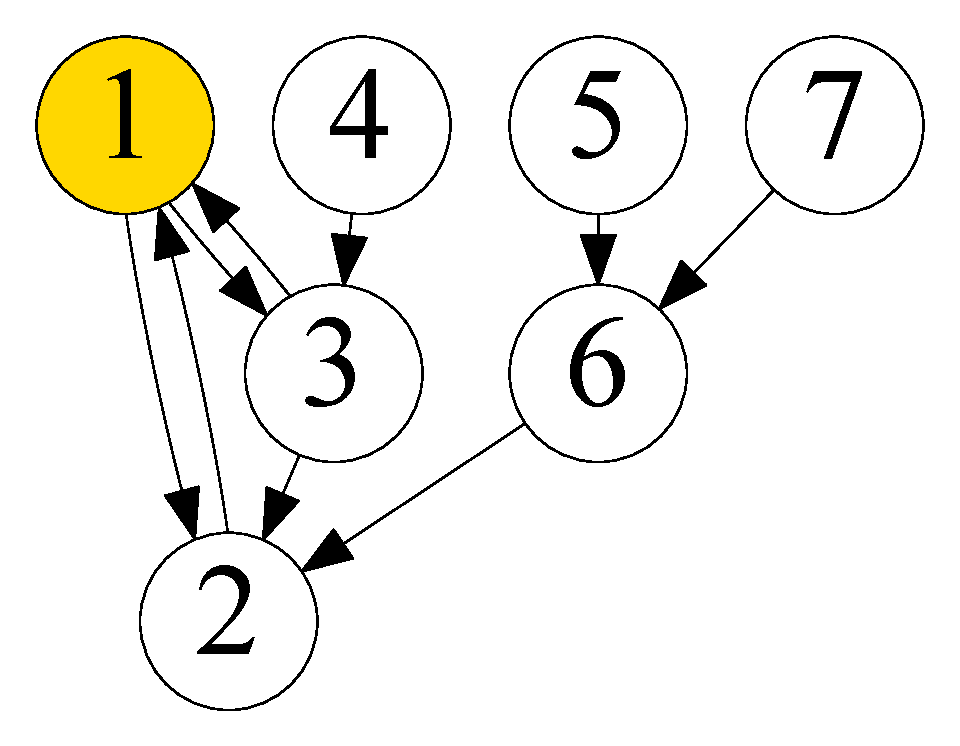
\includegraphics[width=0.5\columnwidth]{./alg_fig/fvs-eg}
	%\vspace{-1em}
	\caption{An example of a directed graph; node 1 forms a feedback vertex set.}
	%\vspace{-1em}
	\label{fig:fvs}
\end{figure}

% dependency graph
%Our algorithms for IBVR are based on a graph representation of the transaction batches. 
How do we compute $B'$? We observe that every batch $B$ of viable transactions 
has an associated \emph{dependency graph} $G$, a directed graph whose nodes are the transactions in $B$ and whose edges are read-write dependencies.
If $G$ is acyclic, then there exists a commit order $Q$ on $G$ that respects all read-write dependencies. We can construct $Q$ by repeatedly committing a transaction whose corresponding node in $G$ has no outgoing edge using a topological sort. 

If $G$ is not acyclic, we can model this problem as an instance of the feedback vertex set problem. 
%show that the of finding a minimal $B'$ is NP-hard by reducing the NP-hard directed feedback vertex set problem 
%to the selection of a minimal $B'$~\cite{karp1972reducibility}. 
A feedback vertex set (FVS) of a directed graph is a subset of vertices whose removal makes the graph acyclic. For example, consider the graph in Figure~\ref{fig:fvs}. Vertex 1 forms a FVS since the graph becomes acyclic after removing Vertex 1 and its incoming and outgoing edges. Finding a minimal-size $B'$ for IBVR is exactly the problem of finding the minimal (smallest-size) feedback vertex set on $G$. If we have a more complex objective function for IBVR, we can assign weights to the nodes to represent the desired transaction priorities, and look for a minimum-weight FVS. 
Once we find the FVS $B'$, removing the nodes in $B'$ from $G$ yields an acyclic graph that determines the desired commit order $Q$.
The directed graph FVS (DFVS) problem is well-studied as it has many applications, including deadlock detection, program verification, and Bayesian inference. Unfortunately, it is NP-hard and APX-hard~\cite{kann1992approximability, karp1972reducibility}, and it is still an open problem whether there exists any constant-factor approximation.
We propose several practical algorithms for finding a FVS in the next section.


%%%%%%%%%%%%%%%%%%%%%%%%%%%%%%%%%%%%%%%%%%%%%%%%%%%%%%%%%%%%%%%%%%%%%%
%%%%%%%%%%%  VALIDATOR BATCHING: OUR ALGORITHMS
%%%%%%%%%%%%%%%%%%%%%%%%%%%%%%%%%%%%%%%%%%%%%%%%%%%%%%%%%%%%%%%%%%%%%%

\section{Validator Batching}
\label{sec:valbatching}
All our IBVR algorithms begin by constructing the dependency graph $G$. 
%We start with a batch of transactions and construct $B$ by discarding all non-viable transactions. We can identify such transactions by validating each transaction against all the updates prior to this batch.
We create one node per transaction, and one edge per read-write dependency. 
To determine whether a read-write dependency holds from transaction $t'$ to $t$, we check whether $WS(t) \cap RS(t') \neq \emptyset$. If so, we add an edge from $t'$ to $t$. We implement this by creating a hash table from the write sets and probing it with the read sets. Since a read in $t$ can potentially conflict with all the other transactions in the batch, the time complexity to probe the hash table for a single read is $O(|B|)$, where $|B|$ is the size of the batch. The complexity of building $G$ is thus $O(|B|^2+|R|+|W|)$, where $|R|$ is the total number of reads, and $|W|$ is the total number of writes. 

We now process $G$ to find a feedback vertex set. Both before and during the
execution of our FVS algorithms, we \emph{trim} the graph to remove all the nodes
that have no incoming edges and/or no outgoing edges since such nodes cannot
participate in any cycles.


\subsection{Algorithms}
\label{subsec:validator_reordering:algorithm}

\begin{algorithm}[t]
	\SetAlgoLined\DontPrintSemicolon
	\SetKwProg{main}{Algorithm}{}{}
	\main{GreedySccGraph($G$, $P$)}{
		\KwIn{Directed graph $G$, policy $P$}
		\KwOut{$V$, a feedback vertex set for $G$}
		$V\gets \emptyset$\;
		$G'\gets trim(G)$\;
		$SCC = StronglyConnectedComponents(G')$\;
		\For {$S \in SCC$} {
			$V\gets V\cup GreedyComponent(S, P)$\;
		}
		\Return{$V$}\;
	}{}
	
	\SetKwProg{sub}{Algorithm}{}{}
	\sub{GreedyComponent($S$, $P$)}{
		\KwIn{SCC $S$, policy $P$}
		\KwOut{$V'$, a feedback vertex set for $S$}
		
		\If {$S.size == 1$} {
			\Return{$\emptyset$}\;
		}
		$v\gets SelectVertexByPolicy(S, P)$\;
		$S'\gets GetGraphAfterVertexRemoval(S, v)$\;
		\Return{$v \cup GreedySccGraph(S', P)$}\;
	}{}
	
	\caption{SCC-based greedy algorithm}
	\label{alg:scc}
\end{algorithm}


\begin{algorithm}[t]
	\SetAlgoLined\DontPrintSemicolon
	\SetKwProg{main}{Algorithm}{}{}
	\main{GreedySortGraph($G$, $P$, $k$)}{
		\KwIn{Directed graph $G$, policy $P$, multi factor $k$}
		\KwOut{$V$, a feedback vertex set for $G$}
		$V\gets \emptyset$\;
		$G\gets trim(G)$\;
		\While {$G\neq \emptyset$} {
			\If {$G.size < k$} {
				$V\gets V\cup GreedySortGraph(G, P, 1)$\;
				break\;
			}
			$Q\gets QuickSelectVertexByPolicy(G, P, k)$\;
			\For {$i=1; i\leq k; ++i$} {
				$V\gets V\cup Q[i]$\;
				$G\gets GetGraphAfterVertexRemoval(G, Q[i])$\;
			}
			$G\gets trim(G)$\;
		}
		\Return{$V$}\;
	}{}
	\caption{Sort-based greedy algorithm}
	\label{alg:sort}
\end{algorithm}

{\bf SCC-Based Greedy Algorithm.} The intuition behind our first algorithm is that each cycle must be contained in a strongly connected component of the graph. After preprocessing, we partition the graph into SCCs. For a graph with $V$ vertices and $E$ edges, we can do this in time $O(|V|+|E|)$ using Tarjan's SCC algorithm~\cite{tarjan1972depth}.

Nodes in SCCs of size one cannot belong to any cycle. For a SCC that contains
more than one node, we choose a vertex to remove according to a \emph{policy}. The policy is a ranking function over vertices, and we greedily choose the top-ranked vertex to remove. We then recurse on the remaining graph. Algorithm~\ref{alg:scc} shows the details of this procedure. We begin by trimming and partitioning the graph into SCCs  (lines 3-4). We process each SCC $S$ using $GreedyComponent(S, P)$ (lines 5-7). This subroutine starts by eliminating SCCs of size one (lines 10-12). Next, it chooses the top-ranked vertex $v$ from $S$ under Policy $P$ (line 13). It removes $v$ from $S$ and recursively calls $GreedySccGraph$ on the remaining graph $S'$ (line 14 - 15). Finally, it returns the union of all the FVSs obtained in processing $S$ (line 15). When the top-level procedure $GreedySccGraph(G, P)$ has processed all the SCCs of $G$, it returns the union of the FVSs obtained (line 8).
% Time complexity analysis
Trimming and updating the graph after removing a node take $O(|V| + |E|)$ per
graph in total, since each node / edge can be removed only once. In the worst case, e.g., in a fully connected graph, we may only remove one node per iteration. Since SCC takes $O(|V|+|E|)$ per iteration, the time complexity of this algorithm is $O(|V|(|V|+|E|))$.
The policy $P$ is at the heart of the algorithm, and it ranks vertices which are likely to be included in a desirable FVS highly. We discuss possible policies in Section \ref{subsec:validator_reordering:policy}.

\begin{figure*}[t]
	\centering
	\begin{minipage}[b]{0.19\linewidth}
		\captionsetup{type=figure}
		\centering
		\subcaptionbox{original\label{fig:scc:g0}}
		{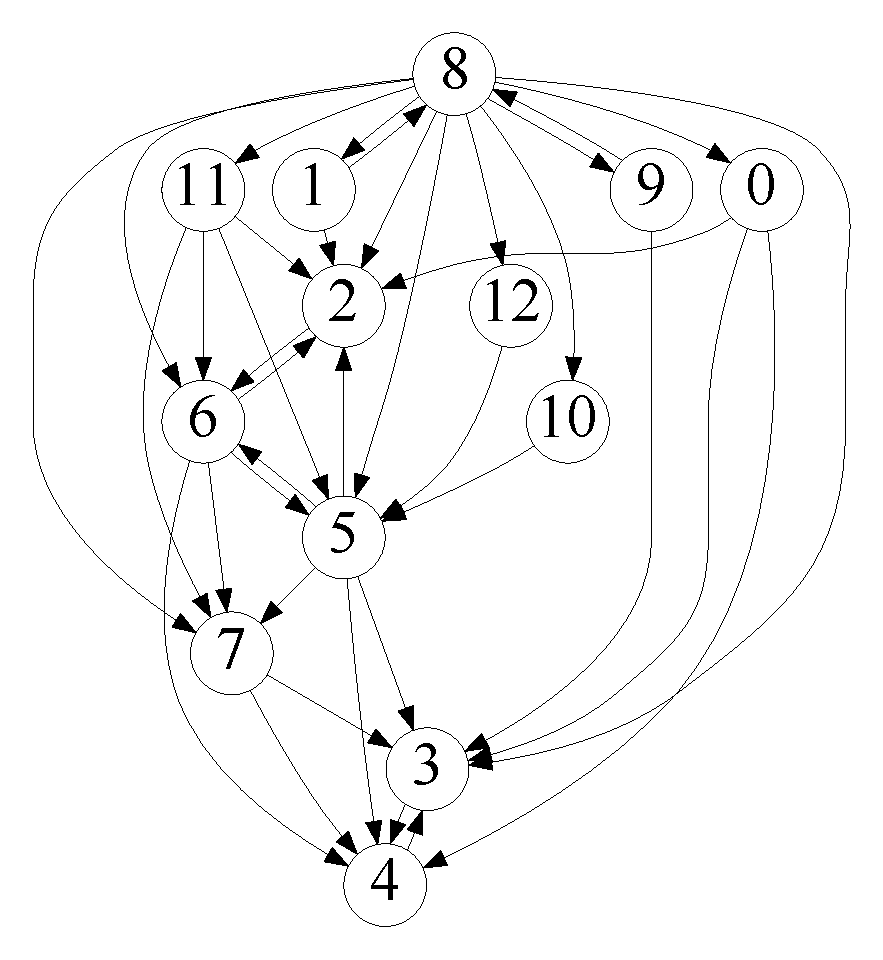
\includegraphics[width=\textwidth]{./alg_fig/scc-g0}}
		%     \vspace{-2em}
	\end{minipage}
	\begin{minipage}[b]{0.19\linewidth}
		\centering
		\subcaptionbox{partition into SCCs\label{fig:scc:g1}}
		{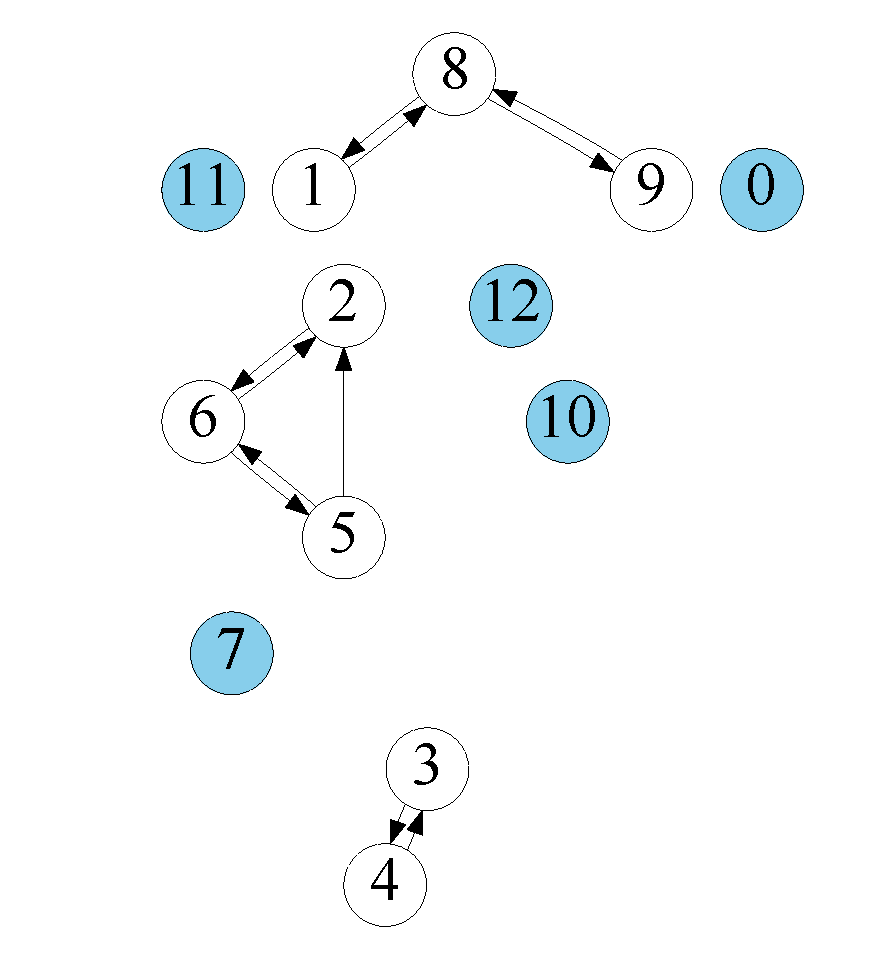
\includegraphics[width=\textwidth]{./alg_fig/scc-g1}}
		%    \vspace{-2em}
	\end{minipage}
	\begin{minipage}[b]{0.19\linewidth}
		\centering
		\subcaptionbox{add 3 to FVS\label{fig:scc:g3}}
		{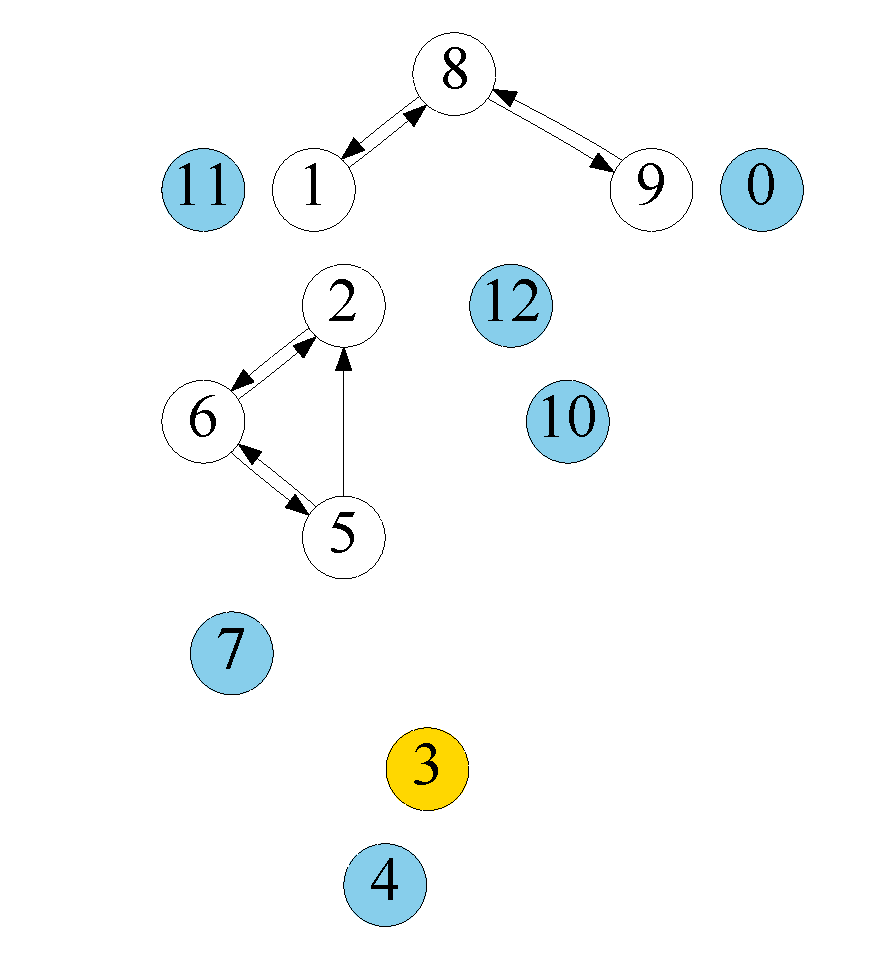
\includegraphics[width=\textwidth]{./alg_fig/scc-g3}}
		%       \vspace{-2em}
	\end{minipage}
	\begin{minipage}[b]{0.19\linewidth}
		\centering
		\subcaptionbox{add 6 to FVS\label{fig:scc:g5}}
		{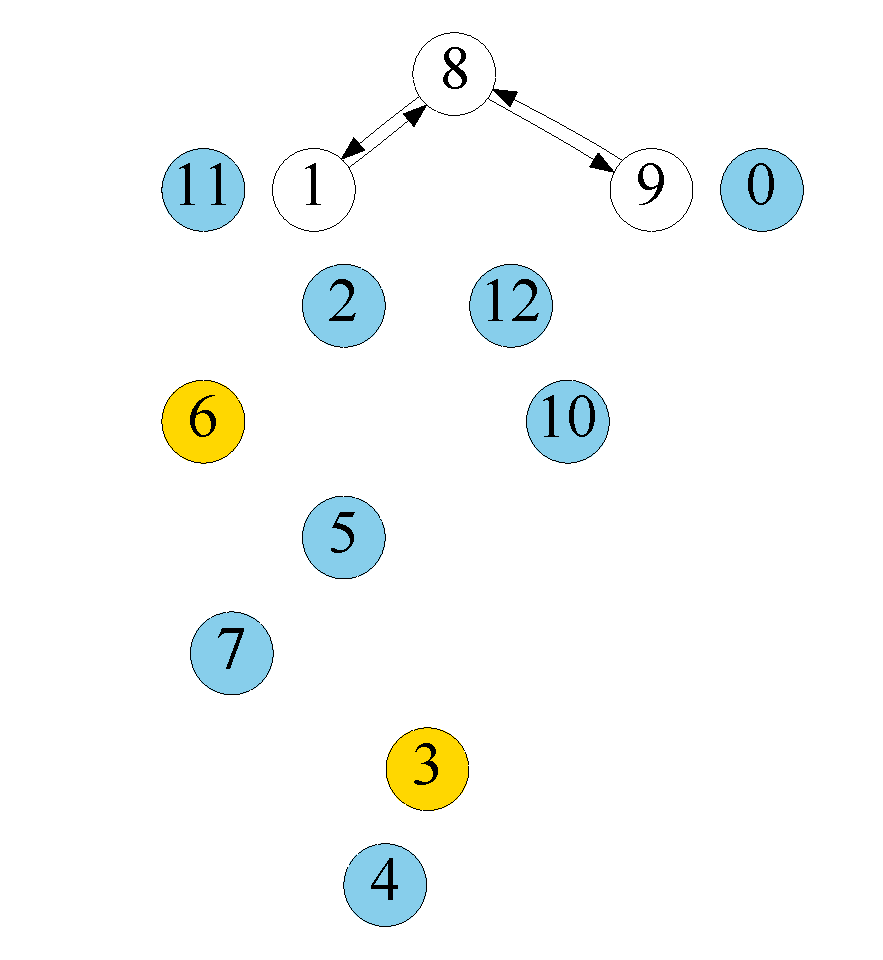
\includegraphics[width=\textwidth]{./alg_fig/scc-g5}}
		%      \vspace{-2em}
	\end{minipage}                  
	\begin{minipage}[b]{0.19\linewidth}
		\centering
		\subcaptionbox{add 8 to FVS\label{fig:scc:g7}}
		{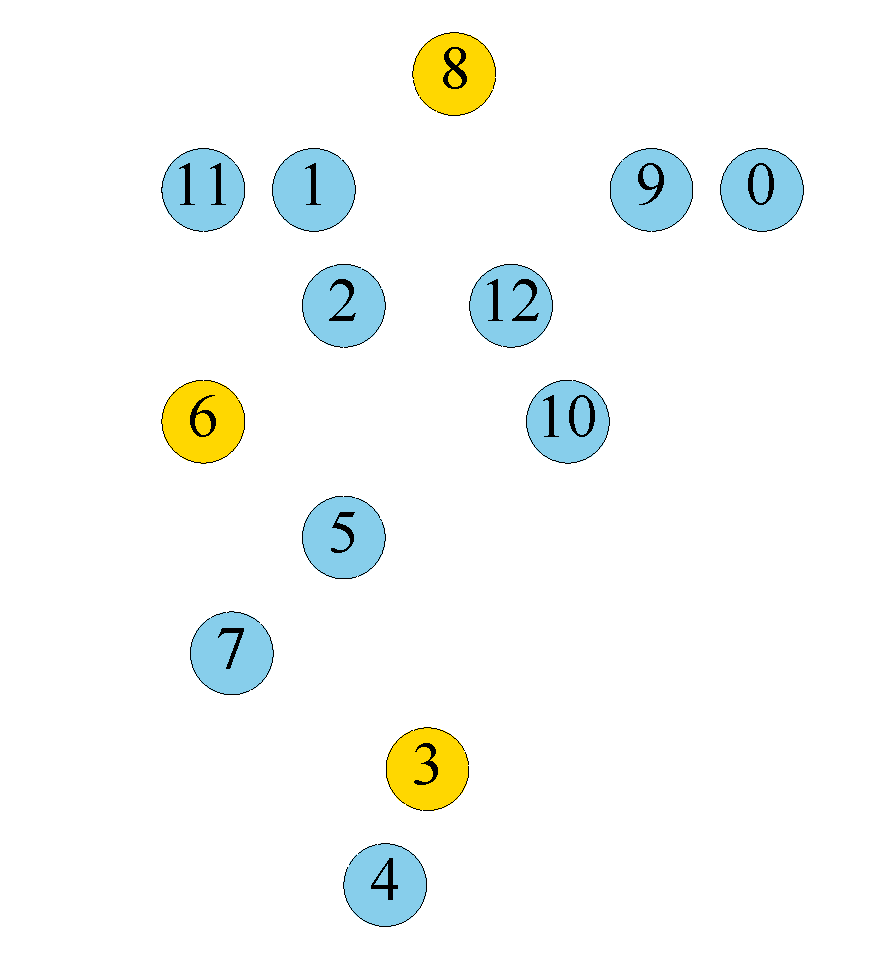
\includegraphics[width=\textwidth]{./alg_fig/scc-g7}}
		%     \vspace{-2em}
	\end{minipage}  
	%\vspace{-1em}             
	\caption{An example of the SCC-based greedy algorithm using \texttt{prod-degree} policy. Blue nodes are trimmed during the algorithm, and yellow nodes form the FVS.}
	%\vspace{-1em}
	\label{fig:scc}
\end{figure*}

{\bf An example.} Figure~\ref{fig:scc} shows an instance of the SCC-based greedy algorithm that aims at minimizing the size of FVS, with a policy $P$ selecting the node with the largest product of its in-degree and out-degree, i.e., \texttt{prod-degree}. The graph cannot be trimmed, so we partition it into SCCs. We remove all SCCs of size 1 --  Nodes 0, 7, 10, 11, and 12 (Figure~\ref{fig:scc:g1}). There are three remaining SCCs. We first look at the component containing Nodes 3 and 4. Since Nodes 3 and 4 have the same product of in-degree and out-degree, we can add either one of them to the FVS. We choose Node 3. Now Node 4 has neither incoming nor outgoing edges, so it is trimmed (Figure~\ref{fig:scc:g3}). We repeat the process with the other components. For the SCC containing Nodes 2, 5, and 6, we add Node 6 to the FVS, as it has the largest product of in-degree and out-degree among the three nodes in this SCC. We now trim Nodes 2 and 5 (Figure~\ref{fig:scc:g5}). Finally, we remove Node 8 from the last component, and trim Nodes 1 and 9 (Figure~\ref{fig:scc:g7}). This leaves us with a final FVS consisting of Nodes 3, 6, and 8.

{\bf Sort-Based Greedy Algorithm.} Our first algorithm relies on a SCC partitioning routine that takes linear time in the size of the graph. As this routine is called several times throughout the algorithm, it can cause a non-trivial overhead. Here we propose a faster greedy algorithm using a sort-based approach to remove nodes. Through extensive empirical tests of the SCC-based greedy algorithm, we found that at each iteration, all the top ranked nodes in the graph are very likely to be included in the final FVS. Our second algorithm is based on this observation; it sorts the nodes according to a policy $P$, and includes the $k$ top-ranked nodes in the FVS. We call $k$ the \emph{multi factor} of the algorithm. The algorithm removes these nodes and iterates on the remaining graph.

Algorithm~\ref{alg:sort} shows this in more detail. We start by trimming the graph (line 3); if the graph has no more than $k$ nodes, we reduce the multi-factor to 1 (line 5-8). Otherwise, we sort and select top ranked $k$ nodes into a queue $Q$ using $P$ with the Quickselect algorithm~\cite{hoare61cacm}, and include the $k$ nodes in $V$ (line 9-13).
After removing the selected nodes from $G$, we trim the remaining graph
again (line 14). We repeat this procedure until the graph is empty (line 4). 
% time complexity analysis.
As with the previous algorithm, updating the graph after removing a node and \emph{trim} takes $O(|V|+|E|)$ in total. Updating the weights of the remaining nodes takes $O(|V|)$ per iteration. The
Quickselect algorithm~\cite{hoare61cacm} has an amortized time complexity of
$O(|V|)$. In the worst case, it will take $O(|V|/k)$ iterations to terminate. So
the overall time complexity is $O(|V|^2/k + |V| + |E|)$.
This algorithm has smaller time complexity than the SCC-based greedy algorithm, and we can increase $k$ to further trade accuracy for shorter runtime. As we will see in Section~\ref{sec:experiments}, it produces results of comparable accuracy to the SCC-based algorithm in practice.

\begin{figure*}[t]
	\centering
	\begin{minipage}[b]{0.19\linewidth}
		\captionsetup{type=figure}
		\centering
		\subcaptionbox{original\label{fig:simple:g0}}
		{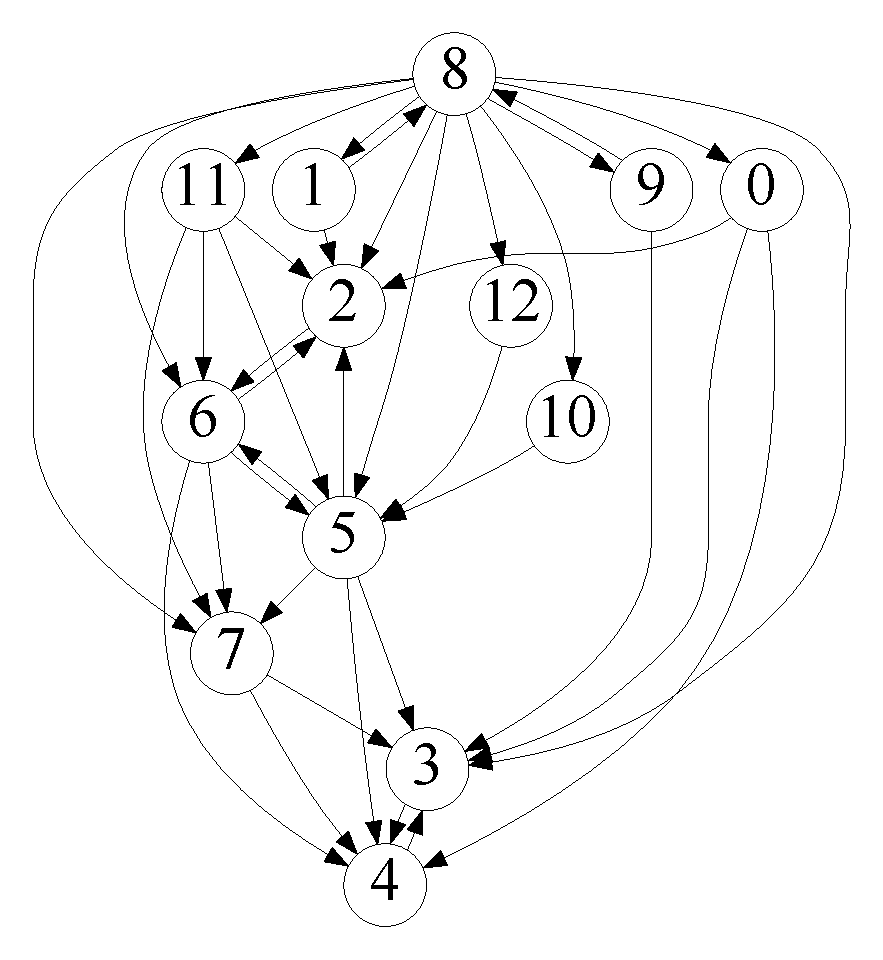
\includegraphics[width=\textwidth]{./alg_fig/simple-g0}}
		%     \vspace{-2em}
	\end{minipage}
	\begin{minipage}[b]{0.19\linewidth}
		\centering
		\subcaptionbox{add 5 to FVS\label{fig:simple:g2}}
		{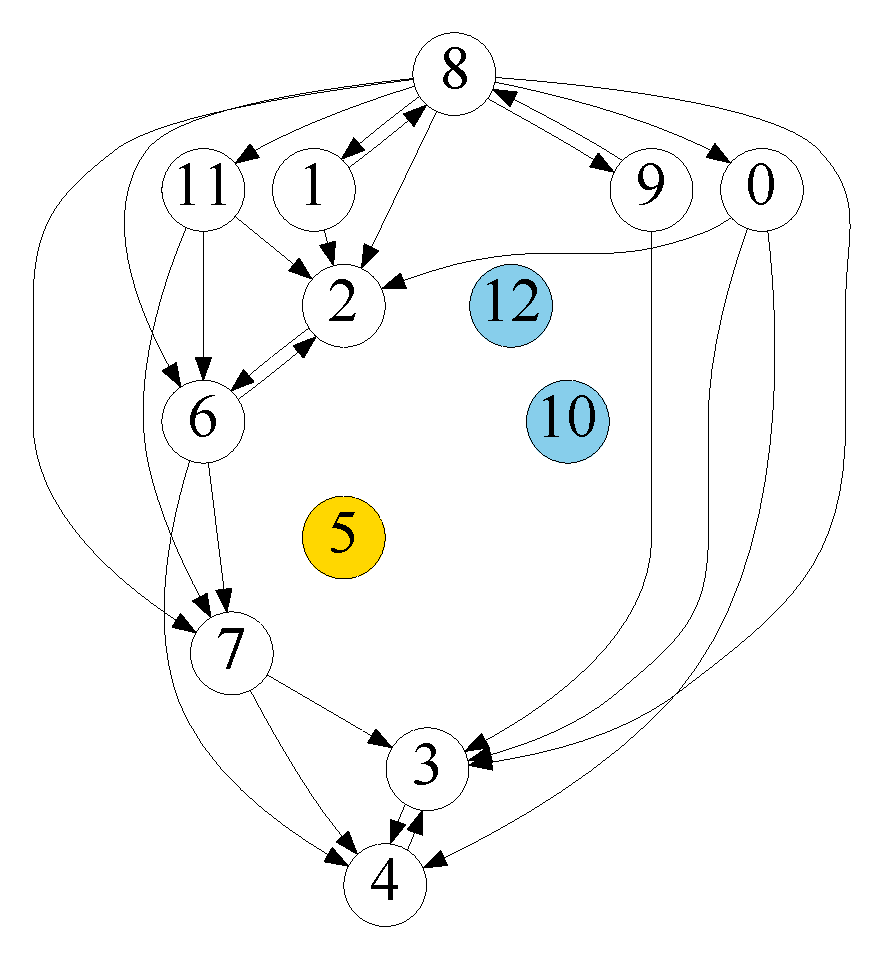
\includegraphics[width=\textwidth]{./alg_fig/simple-g2}}
		%    \vspace{-2em}
	\end{minipage}
	\begin{minipage}[b]{0.19\linewidth}
		\centering
		\subcaptionbox{add 8 to FVS\label{fig:simple:g4}}
		{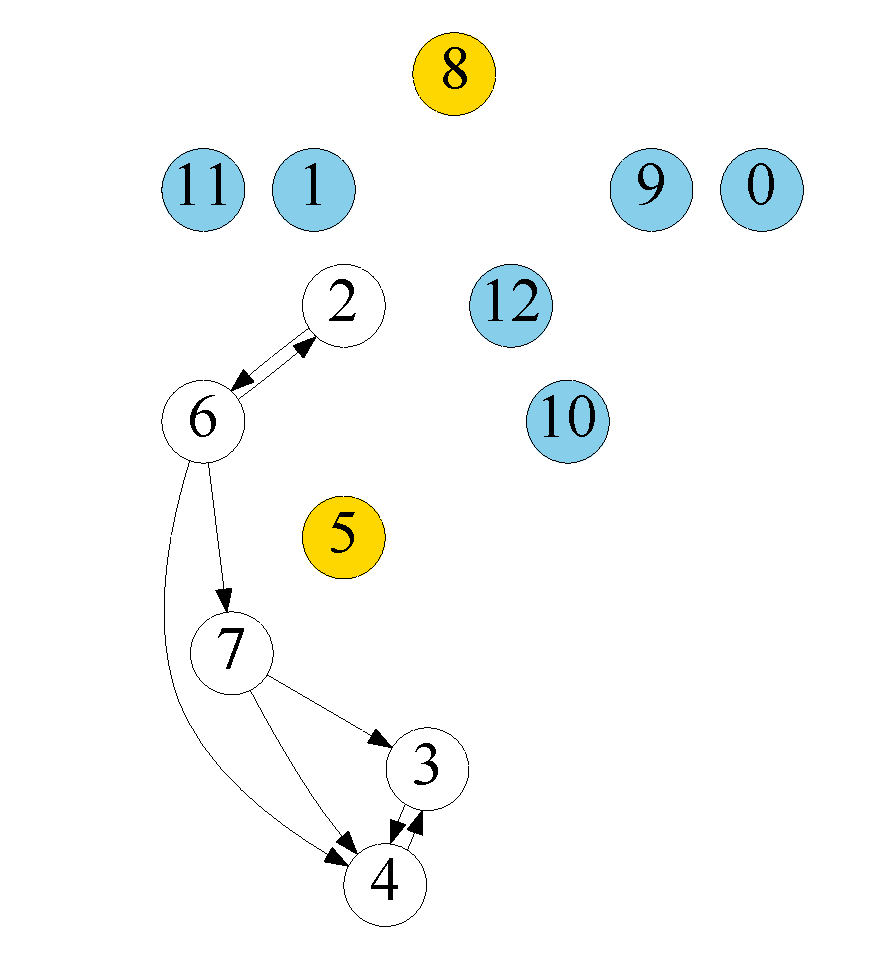
\includegraphics[width=\textwidth]{./alg_fig/simple-g4}}
		%       \vspace{-2em}
	\end{minipage}
	\begin{minipage}[b]{0.19\linewidth}
		\centering
		\subcaptionbox{add 6 to FVS\label{fig:simple:g6}}
		{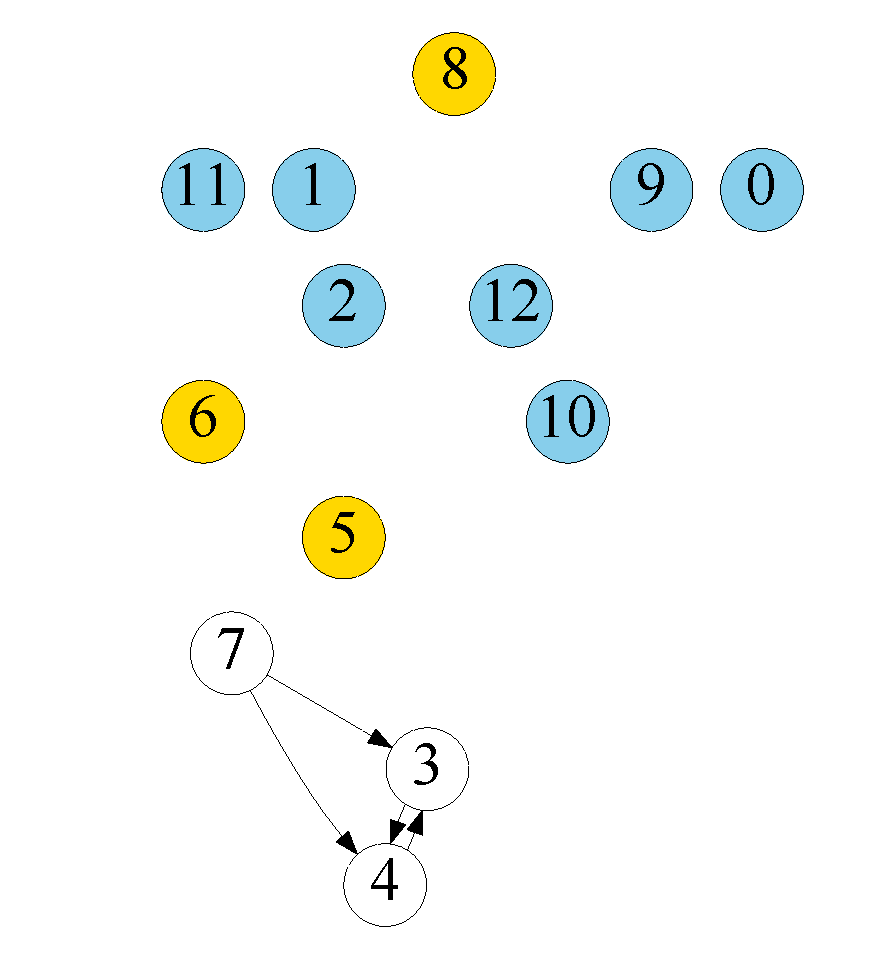
\includegraphics[width=\textwidth]{./alg_fig/simple-g6}}
		%      \vspace{-2em}
	\end{minipage}                  
	\begin{minipage}[b]{0.19\linewidth}
		\centering
		\subcaptionbox{add 3 to FVS\label{fig:simple:g8}}
		{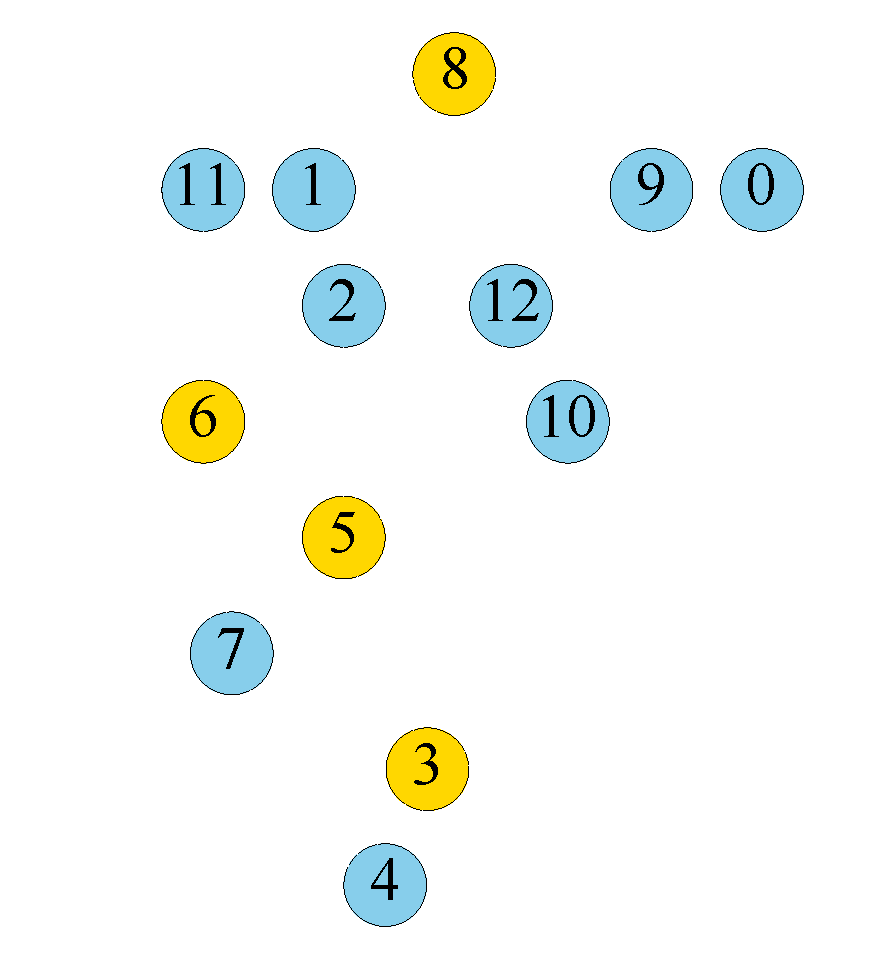
\includegraphics[width=\textwidth]{./alg_fig/simple-g8}}
		%     \vspace{-2em}
	\end{minipage}
	%\vspace{-1em}             
	\caption{An example of the sort-based greedy algorithm using \texttt{prod-degree} policy and multi factor 1. Blue nodes are trimmed during the algorithm, and yellow nodes form the FVS.}
	\label{fig:simple}               
	%\vspace{-1em}    	
\end{figure*}

{\bf Example (Continued).} Figure~\ref{fig:simple} shows the same example using the sort-based greedy algorithm, with $k = 1$. After the first sort, we add Node 5 to the FVS since it has the highest product of in-degree and out-degree. After eliminating Node 5, Nodes 10 and 12 have only incoming edges, and get trimmed (Figure~\ref{fig:simple:g2}). We sort the remaining nodes. This time, we add Node 8 to the FVS, and trim Nodes 0, 1, 9, 11 (Figure~\ref{fig:simple:g4}). We repeat this process with the remaining nodes until the graph is empty. This yields a FVS consisting of Nodes 3, 5, 6, and 8 (Figure~\ref{fig:simple:g8}), which contains one more vertex than the FVS we obtained with the SCC-based algorithm.

{\bf Hybrid Algorithm.}
%\subsubsection{Hybrid algorithm} 
We can combine the SCC-based greedy algorithm and the precise brute-force FVS search into a \emph{hybrid algorithm}. The algorithm is similar to the SCC-based greedy algorithm but runs a precise, brute-force FVS search whenever it can afford to. Instead of processing all SCCs via the $GreedyComponent$ subroutine (lines 5-7 of Algorithm~\ref{alg:scc}), it runs the precise search when processing SCCs that are smaller than a certain \emph{threshold}, and the greedy subroutine $GreedyComponent$ on SCCs that are larger than the threshold. Adjusting the threshold allows us to trade off precision versus runtime.

%%%%%%%%%%%%%%%%%%%%%%%%%%%%%%%%%%%%%%%%%%%%%%%%%%%%%%%%%%%%%%%
\subsection{Policies}
\label{subsec:validator_reordering:policy}
Policies are of utmost importance for our algorithms. Recall that a policy is a ranking function on vertices of the graph, and a good policy ranks vertices which are likely to be in a desirable FVS highly. \changed{We discuss three kinds of policies for different performance objectives and system architectures.}

% minimize number of conflicts
\changed{{\bf Minimize the number of aborts.}}
We first discuss policies that aim at minimizing the number of conflicts, i.e., the size of the FVS. The simplest such policy is \texttt{random} that assigns all nodes random rankings. Alternatively, we can rank nodes using degree-based heuristics, based on the intuition that the removal of a node will break many cycles if the node is high in some measurement of its graph degree. Such heuristics have  been shown to work well for FVS computation~\cite{cutello2015targeting}. For example, the policy \texttt{max-degree} chooses the node with the largest degree (either in-degree or out-degree), \texttt{sum-degree} chooses the node with the largest total degree (in-degree plus out-degree), and \texttt{prod-degree} chooses the node with the largest product of in-degree and out-degree. 

\changed{{\bf Minimize tail latency.}}
% minimize tail latency
More sophisticated policies are possible if the system is optimizing for a metric beyond maximizing the number of commits. For example, we may want to bound the transactions' tail latency; we can do that by incorporating latency information in our policies. We can rank transactions based on how many times they have been aborted and restarted; thus, transactions that have been restarted many times are much less likely to enter the FVS and have a higher chance of committing. Alternatively, we can also devise policies that combine the information about a transaction's number of restarts and its graph degree. For example, we can compute the ranking of a vertex as the product of its in-degree and out-degree divided by an exponential function of the number of restarts of the corresponding transaction. 
% help with transactions with monetary value
%\eat{We can also devise policies that handle hard transactions. In many workloads some transactions are naturally more prone to conflicts, e.g., those that access many objects and/or ``hot'' objects. If we use graph degree based policies, such transactions are likely to be included in the FVS and aborted repeatedly. To avoid starvation, we can adjust our policies to increase the probability that these transactions can commit. For example, we can approximate the ``hardness'' of a transaction by the size of its read and write sets and include that as a weighting factor in the policy.}
In business applications, the monetary value of different transactions varies. Optimizing for maximal monetary value, we can design policies that favor more valuable transactions. For example, we can customize the policy to always add a transaction with the lowest value to the FVS until the resulting dependency graph is acyclic.



\changed{
	%{\bf Thread-aware reordering.}
	{\bf Reduce inter-thread conflicts.}
	Many recent OCC-based OLTP systems use a decentralized architecture~\cite{lim2017cicada, tu2013speedy, yu2016tictoc, kim2016ermia}, where there is no centralized validation.  
	%for validation or storage access. 
	Each transaction is scheduled to a dedicated \emph{thread} and processed by this thread synchronously for its entire lifetime. Since a transaction is executed synchronously, it can only conflict with transactions executed by other threads. 
	
	
	In such an architecture, while batching operations across transactions does not apply, we can assign transactions to threads to reduce inter-thread conflicts. Intuitively, for a batch of incoming transactions, we schedule conflicting transactions to execute on the same thread where they are processed serially. Because conflicting transactions access the same objects, reordering also improves caching within a thread.
	
	We extend our sort-based algorithm to a \emph{thread-aware policy} which assigns transactions thread by thread. We batch a number of transactions and assign the same number of transactions to each thread.\footnote{More sophisticated assignments are possible, but we leave them for future work.} At each thread, we compute the weight of a transaction first based on the number of conflicts to the set of transactions $T$ in the batch that have already been assigned to this thread, then the number of object accesses shared between this transaction and $T$, and finally its number of conflicts to the unassigned transactions in this batch. For each thread, our sort-based algorithm will first pick the transaction with the most conflicts against the remaining transactions, and then it iteratively updates the weights of the transactions left to pick the next one with the highest weight. This policy greedily puts conflicting transactions on the same thread to minimize conflicts across threads; as a side effect, it tries to assign transactions accessing the same objects to the same thread, resulting in better caching. As we will see later in our experiments (Section \ref{sec:OtherOLTP}), this simple policy significantly improves throughput and reduces tail latency.
}% end changed

